\documentclass[border=10pt]{standalone}

\usepackage{tikz}
\usepackage{tikzsymbols}
\usetikzlibrary{calc,patterns,shapes.geometric}

\def\centerarc[#1](#2)(#3:#4:#5){\draw[#1] ($(#2)+({#5*cos(#3)},{#5*sin(#3)})$) arc (#3:#4:#5);}

\begin{document}
	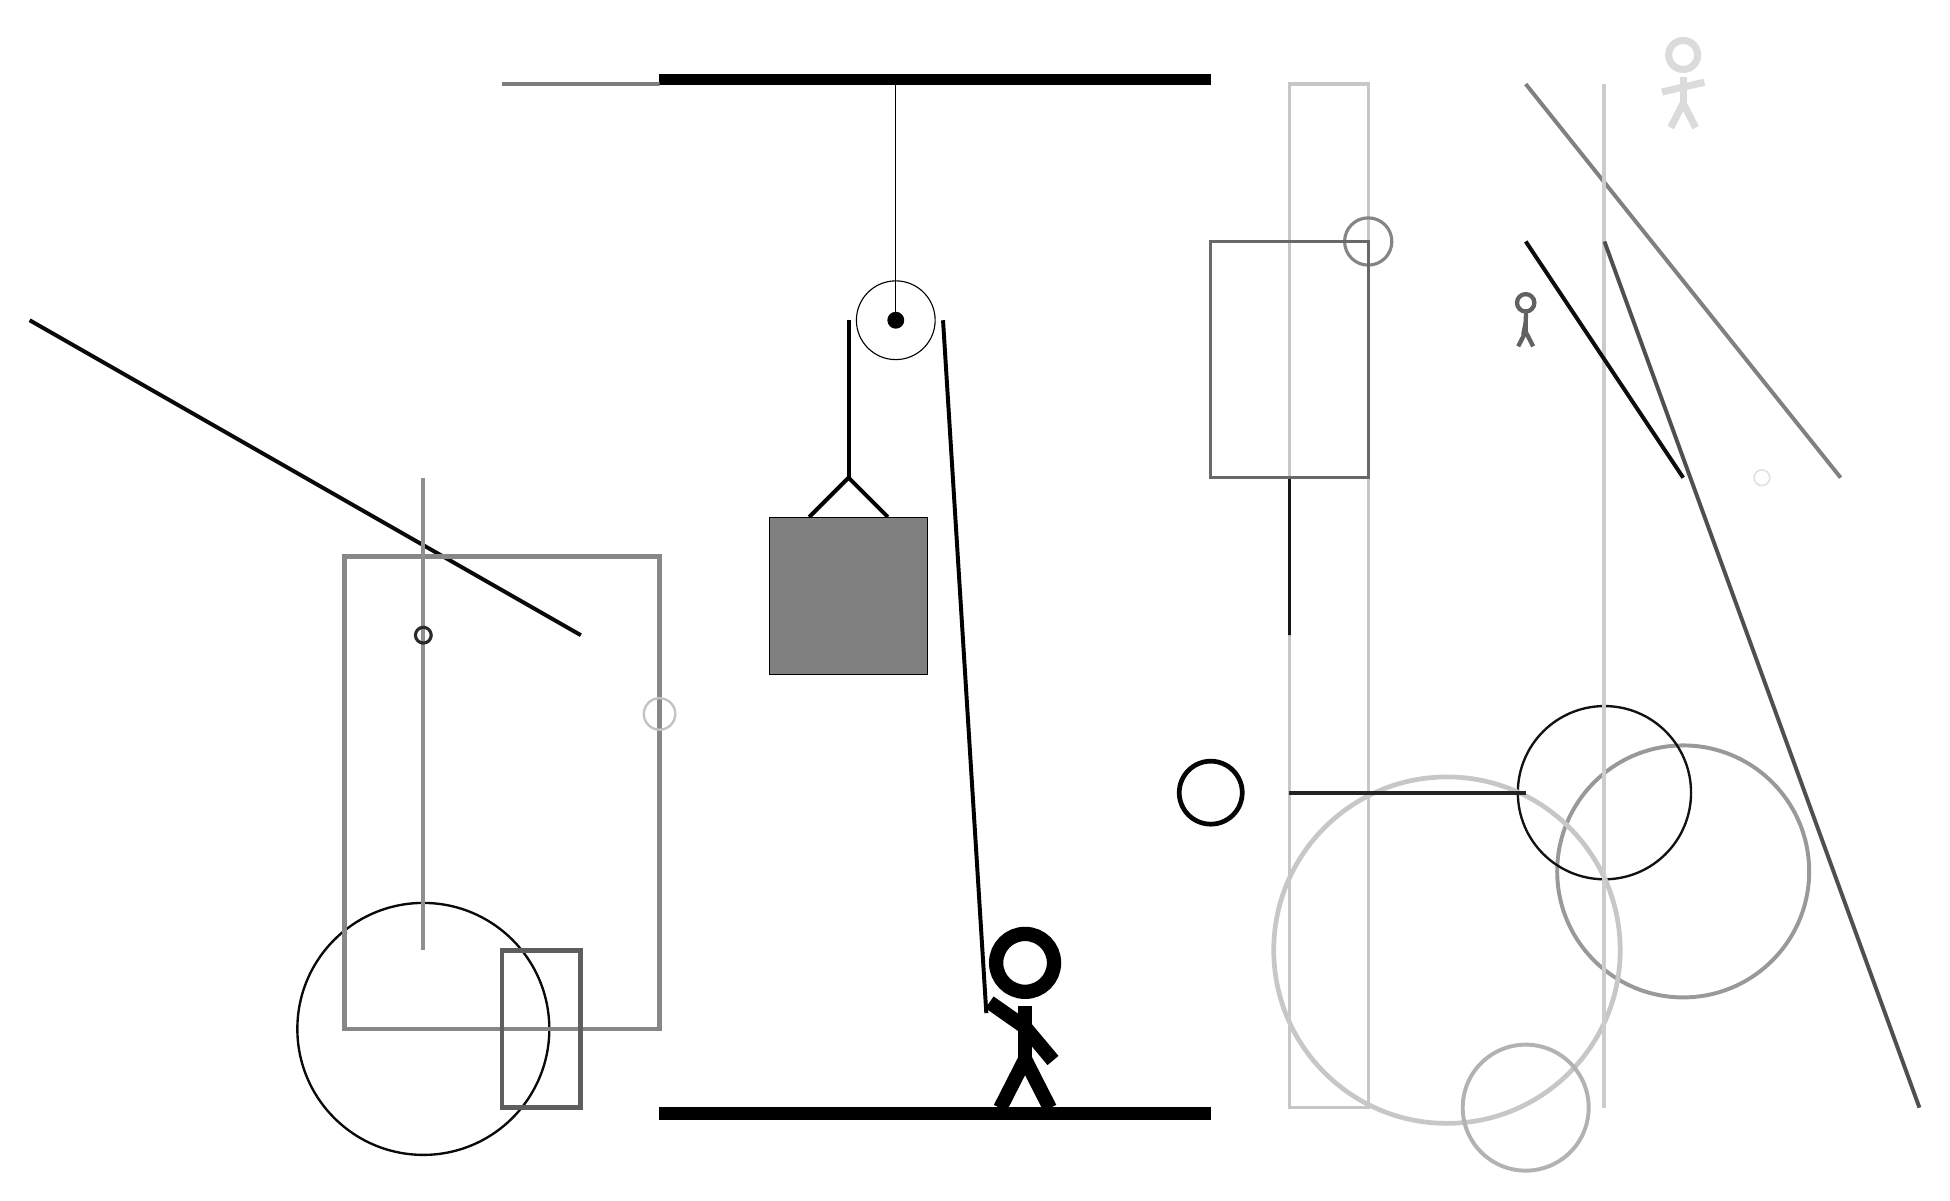
\begin{tikzpicture}
		%%%%% START %%%%%
		
		\draw[fill=black] (-2, 10) rectangle (5, 10.125);
		
		\draw[line width=0.4mm, color=black!51] (-4, 10) rectangle (-2, 10);
		
		\draw [line width=0.5mm, color=black!40](11, 0) circle (1.6);
		\draw [line width=0.3mm, color=black!96](-5, -2) circle (1.6);
		\draw[line width=0.5mm, color=black!50](9, 10) -- (13, 5);
		
		\draw[line width=0.4mm, color=black!22] (6, -3) rectangle (7, 10);
		\draw [line width=0.6mm, color=black!98](5, 1) circle (0.4);
		\draw [line width=0.3mm, color=black!93](10, 1) circle (1.1);
		\draw [line width=0.6mm, color=black!22](8, -1) circle (2.2);
		\draw [line width=0.2mm, color=black!12](12, 5) circle (0.1);
		\draw[line width=0.5mm, color=black!96](-3, 3) -- (-10, 7);
		\draw [line width=0.5mm, color=black!30](9, -3) circle (0.8);
		\node[line width=0.2mm, color=black!14] at (11, 10) {\Strichmaxerl[5][13][13]};
		\draw[line width=0.5mm, color=black!20](10, 10) -- (10, -3);
		
		\draw[line width=0.5mm, color=black!86](9, 1) -- (6, 1);
		\draw[line width=0.6mm, color=black!47] (-2, -2) rectangle (-6, 4);
		\draw[line width=0.5mm, color=black!44](-5, 5) -- (-5, -1);
		
		\draw [line width=0.4mm, color=black!48](7, 8) circle (0.3);
		
		\draw [line width=0.4mm, color=black!83](-5, 3) circle (0.1);
		\draw[line width=0.5mm, color=black!91] (6, 3) rectangle (6, 5);
		\node[line width=0.6mm, color=black!62] at (9, 7) {\Strichmaxerl[3][79][88]};
		\draw[line width=0.5mm, color=black!69](10, 8) -- (14, -3);
		\draw[line width=0.5mm, color=black!95](9, 8) -- (11, 5);
		\draw[line width=0.6mm, color=black!63] (-3, -3) rectangle (-4, -1);
		\draw [line width=0.3mm, color=black!24](-2, 2) circle (0.2);
		\draw[line width=0.4mm, color=black!59] (5, 8) rectangle (7, 5);
		
		\draw (1, 7) circle (0.5);
		\draw[fill=black] (1, 7) circle (0.1);
		\draw (1, 10) -- (1, 7);
		
		\draw[line width=0.5mm] (-0.1, 4.5) -- (0.4, 5.0) -- (0.9, 4.5);
		\draw[fill=black!50] (-0.6, 4.5) rectangle (1.4, 2.5);
		
		\draw[line width=0.5mm] (0.4, 7) -- (0.4, 5.0);
		\centerarc[line width=0.5mm](1, 7)(0:180:0.6);
		\draw[line width=0.5mm](1.6, 7) -- (2.15, -1.8);
		
		\node at (2.6, -1.9) {\Strichmaxerl[10][-35][-50]};
		
		\draw[fill=black] (-2, -3) rectangle (5, -3.15);
		
		%%%%% END %%%%%
	\end{tikzpicture}
\end{document}